%!TEX program = pdflatex
\documentclass[aspectratio=169,10pt]{beamer}

% Theme and colors
\usetheme{metropolis}
\usepackage{appendixnumberbeamer}
\usepackage{booktabs}
\usepackage{graphicx}
\usepackage{tikz}
\usepackage{amsmath}
\usepackage{xcolor}
\usepackage{fontawesome5}
\usepackage{pgfplots}
\pgfplotsset{compat=1.18}
\usetikzlibrary{shapes.geometric, arrows, positioning, calc, decorations.pathreplacing}

% Custom colors matching the paper
\definecolor{criticalred}{RGB}{220,53,69}
\definecolor{warningorange}{RGB}{255,193,7}
\definecolor{safegreen}{RGB}{40,167,69}
\definecolor{accentblue}{RGB}{0,123,255}
\definecolor{darkgray}{RGB}{52,58,64}
\definecolor{lightgray}{RGB}{248,249,250}

% Set metropolis theme colors
\setbeamercolor{frametitle}{bg=darkgray}
\setbeamercolor{progress bar}{fg=accentblue}
\setbeamercolor{alerted text}{fg=criticalred}

% Custom commands
\newcommand{\highlight}[1]{\textcolor{accentblue}{\textbf{#1}}}
\newcommand{\critical}[1]{\textcolor{criticalred}{\textbf{#1}}}
\newcommand{\warning}[1]{\textcolor{warningorange}{\textbf{#1}}}
\newcommand{\safe}[1]{\textcolor{safegreen}{\textbf{#1}}}

% Hide notes for audience version
\setbeameroption{hide notes}

% Metadata
\title{Real-Time Pedestrian-Vehicle Collision Risk Assessment}
\subtitle{Using Physics-Based Trajectory Analysis and Multi-Modal Computer Vision}
\author{Veer Daliya}
\institute{Inspirit AI Research Program}
\date{2024}

\begin{document}

% ============================================================================
% TITLE SLIDE
% ============================================================================
\begin{frame}
\titlepage
\end{frame}

% ============================================================================
% OUTLINE
% ============================================================================
\begin{frame}{Agenda}
\begin{enumerate}
    \item \textbf{Motivation:} Why pedestrian safety matters
    \item \textbf{Problem:} The technical challenges
    \item \textbf{Solution:} Our multi-stage pipeline
    \item \textbf{Key Innovations:} What makes our approach unique
    \item \textbf{Results:} Performance and real-world impact
    \item \textbf{Demo \& Future Work}
\end{enumerate}
\end{frame}

% ============================================================================
% MOTIVATION
% ============================================================================
\begin{frame}{The Problem: Pedestrian Safety Crisis}
\begin{columns}[T]
\begin{column}{0.5\textwidth}
\textbf{Global Statistics:}
\begin{itemize}
    \item \critical{1.35 million} road traffic deaths annually
    \item Pedestrians: \critical{23\%} of all fatalities
    \item \highlight{90\%} of deaths in developing countries
\end{itemize}

\vspace{0.5cm}
\textbf{Current Limitations:}
\begin{itemize}
    \item Human operators can't monitor 24/7
    \item Reactive, not proactive
    \item No early warning capability
\end{itemize}
\end{column}
\begin{column}{0.5\textwidth}
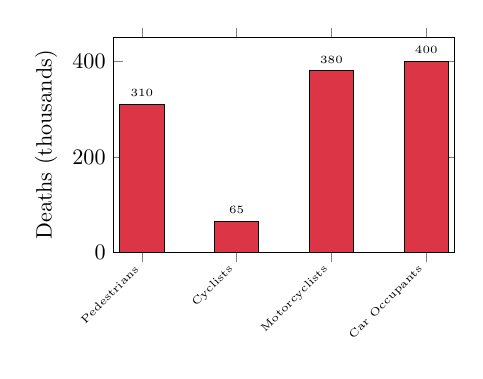
\begin{tikzpicture}[scale=0.8]
\begin{axis}[
    ybar,
    width=7cm,
    height=5cm,
    bar width=20pt,
    ylabel={Deaths (thousands)},
    symbolic x coords={Pedestrians, Cyclists, Motorcyclists, Car Occupants},
    xtick=data,
    x tick label style={rotate=45, anchor=east, font=\tiny},
    nodes near coords,
    nodes near coords style={font=\tiny},
    ymin=0,
    ymax=450,
]
\addplot[fill=criticalred] coordinates {
    (Pedestrians, 310)
    (Cyclists, 65)
    (Motorcyclists, 380)
    (Car Occupants, 400)
};
\end{axis}
\end{tikzpicture}
\end{column}
\end{columns}
\end{frame}

% ============================================================================
% VISION
% ============================================================================
\begin{frame}{Our Vision: Proactive Collision Prevention}
\begin{center}
\begin{tikzpicture}[
    box/.style={rectangle, rounded corners, draw=darkgray, fill=lightgray,
                minimum width=3cm, minimum height=1.5cm, align=center, font=\small},
    arrow/.style={->, >=stealth, thick, color=accentblue}
]
    % Boxes
    \node[box] (detect) at (0,0) {\faCamera\\Detection};
    \node[box] (track) at (4,0) {\faRoute\\Tracking};
    \node[box] (predict) at (8,0) {\faBrain\\Prediction};
    \node[box] (alert) at (12,0) {\faBell\\Alert};

    % Arrows
    \draw[arrow] (detect) -- (track);
    \draw[arrow] (track) -- (predict);
    \draw[arrow] (predict) -- (alert);

    % Time annotations
    \node[below=0.5cm of detect, font=\tiny, color=darkgray] {Frame 0};
    \node[below=0.5cm of predict, font=\tiny, color=darkgray] {t = now};
    \node[below=0.5cm of alert, font=\tiny, color=criticalred] {\textbf{1.5-3s before collision}};
\end{tikzpicture}
\end{center}

\vspace{0.5cm}
\begin{center}
\Large\highlight{Goal: Provide 1.5--3 seconds of advance warning}

\normalsize
Enough time for braking or evasive action
\end{center}
\end{frame}

% ============================================================================
% TECHNICAL CHALLENGES
% ============================================================================
\begin{frame}{Technical Challenges}
\begin{columns}[T]
\begin{column}{0.5\textwidth}
\textbf{Challenge 1: Real-Time Performance}
\begin{itemize}
    \item Process 10+ frames per second
    \item End-to-end latency $<$ 100ms
    \item Run on consumer hardware
\end{itemize}

\vspace{0.3cm}
\textbf{Challenge 2: Stable Tracking}
\begin{itemize}
    \item Maintain identity across occlusions
    \item Handle crowded scenes
    \item Support PTZ camera motion
\end{itemize}
\end{column}
\begin{column}{0.5\textwidth}
\textbf{Challenge 3: Metric-Space Prediction}
\begin{itemize}
    \item Convert pixels to meters
    \item No camera calibration available
    \item Variable scene geometry
\end{itemize}

\vspace{0.3cm}
\textbf{Challenge 4: False Positive Control}
\begin{itemize}
    \item Passengers inside vehicles
    \item Parallel motion (no collision risk)
    \item Brief proximity without danger
\end{itemize}
\end{column}
\end{columns}
\end{frame}

% ============================================================================
% SYSTEM ARCHITECTURE
% ============================================================================
\begin{frame}{System Architecture Overview}
\begin{center}
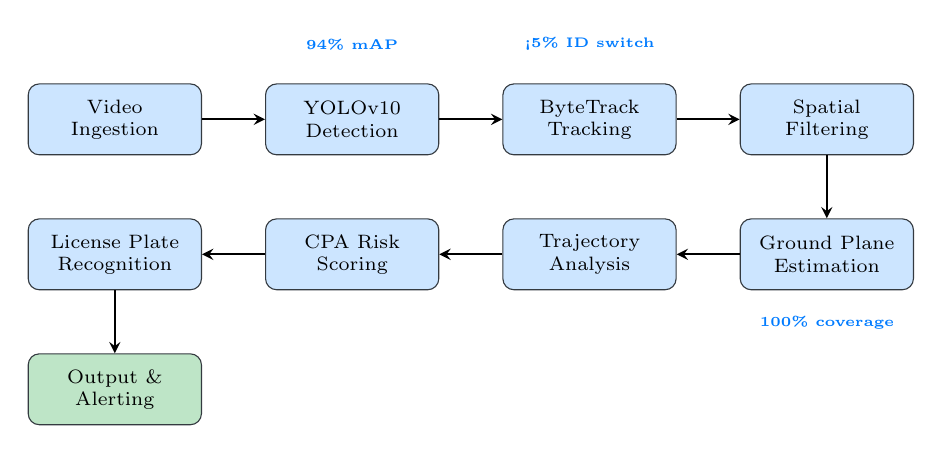
\begin{tikzpicture}[
    node distance=0.8cm,
    module/.style={rectangle, rounded corners, draw=darkgray, fill=accentblue!20,
                   minimum width=2.2cm, minimum height=0.9cm, align=center, font=\scriptsize},
    arrow/.style={->, >=stealth, thick}
]
    % Row 1
    \node[module] (ingest) {Video\\Ingestion};
    \node[module, right=of ingest] (detect) {YOLOv10\\Detection};
    \node[module, right=of detect] (track) {ByteTrack\\Tracking};
    \node[module, right=of track] (filter) {Spatial\\Filtering};

    % Row 2
    \node[module, below=of filter] (ground) {Ground Plane\\Estimation};
    \node[module, left=of ground] (traj) {Trajectory\\Analysis};
    \node[module, left=of traj] (cpa) {CPA Risk\\Scoring};
    \node[module, left=of cpa] (lpr) {License Plate\\Recognition};

    % Row 3
    \node[module, below=of lpr, fill=safegreen!30] (output) {Output \&\\Alerting};

    % Arrows
    \draw[arrow] (ingest) -- (detect);
    \draw[arrow] (detect) -- (track);
    \draw[arrow] (track) -- (filter);
    \draw[arrow] (filter) -- (ground);
    \draw[arrow] (ground) -- (traj);
    \draw[arrow] (traj) -- (cpa);
    \draw[arrow] (cpa) -- (lpr);
    \draw[arrow] (lpr) -- (output);

    % Labels
    \node[above=0.3cm of detect, font=\tiny\bfseries, color=accentblue] {94\% mAP};
    \node[above=0.3cm of track, font=\tiny\bfseries, color=accentblue] {<5\% ID switch};
    \node[below=0.2cm of ground, font=\tiny\bfseries, color=accentblue] {100\% coverage};
\end{tikzpicture}
\end{center}
\end{frame}

% ============================================================================
% INNOVATION 1: GROUND PLANE
% ============================================================================
\begin{frame}{Key Innovation \#1: Ground Plane Estimation Cascade}
\begin{columns}[T]
\begin{column}{0.55\textwidth}
\textbf{The Problem:}\\
Need metric coordinates without camera calibration

\vspace{0.4cm}
\textbf{Our Solution: Three-Method Cascade}
\begin{enumerate}
    \item \highlight{Lane-Based} (most accurate)
    \begin{itemize}
        \item Detect lane markings
        \item Compute vanishing point
        \item Derive homography
    \end{itemize}
    \item \highlight{Horizon-Based} (good fallback)
    \begin{itemize}
        \item Detect horizon line
        \item Estimate camera pitch
    \end{itemize}
    \item \highlight{Size-Based} (always works)
    \begin{itemize}
        \item Use pedestrian height (1.7m)
        \item Geometric projection
    \end{itemize}
\end{enumerate}
\end{column}
\begin{column}{0.45\textwidth}
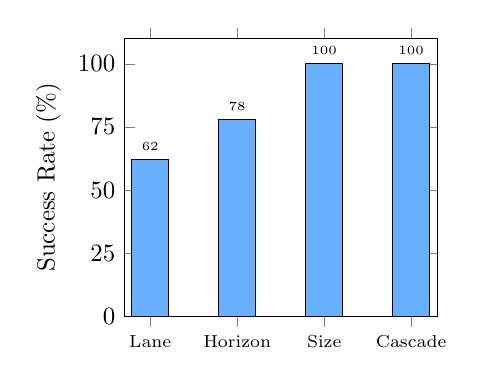
\begin{tikzpicture}[scale=0.9]
\begin{axis}[
    ybar,
    width=6cm,
    height=5.5cm,
    bar width=15pt,
    ylabel={Success Rate (\%)},
    symbolic x coords={Lane, Horizon, Size, Cascade},
    xtick=data,
    x tick label style={font=\scriptsize},
    nodes near coords,
    nodes near coords style={font=\tiny},
    ymin=0,
    ymax=110,
    ytick={0,25,50,75,100},
]
\addplot[fill=accentblue!60] coordinates {
    (Lane, 62)
    (Horizon, 78)
    (Size, 100)
    (Cascade, 100)
};
\end{axis}
\end{tikzpicture}

\vspace{0.2cm}
\centering\small
\highlight{100\% coverage} with \highlight{1.1m} mean error
\end{column}
\end{columns}
\end{frame}

% ============================================================================
% INNOVATION 2: CPA
% ============================================================================
\begin{frame}{Key Innovation \#2: Physics-Based Collision Prediction}
\begin{columns}[T]
\begin{column}{0.55\textwidth}
\textbf{Closest Point of Approach (CPA)}

Classical physics for collision avoidance:

\vspace{0.3cm}
\textbf{Time to closest approach:}
\begin{equation*}
t_{CPA} = -\frac{(\mathbf{p}_p - \mathbf{p}_v) \cdot (\mathbf{v}_p - \mathbf{v}_v)}{|\mathbf{v}_p - \mathbf{v}_v|^2}
\end{equation*}

\vspace{0.2cm}
\textbf{Minimum separation:}
\begin{equation*}
d_{min} = |(\mathbf{p}_p - \mathbf{p}_v) + t_{CPA} \cdot (\mathbf{v}_p - \mathbf{v}_v)|
\end{equation*}

\vspace{0.3cm}
\textbf{Advantages:}
\begin{itemize}
    \item Interpretable predictions
    \item No training data required
    \item Guaranteed behavior
\end{itemize}
\end{column}
\begin{column}{0.45\textwidth}
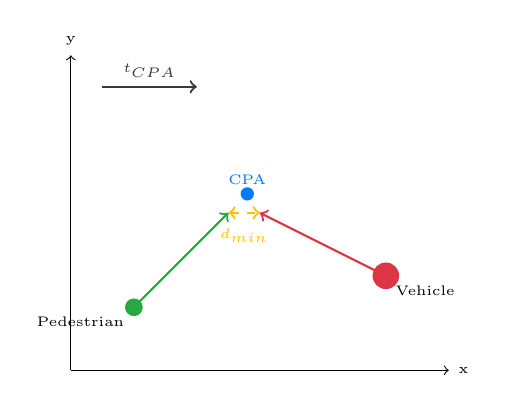
\begin{tikzpicture}[scale=0.8]
    % Coordinate system
    \draw[->] (0,0) -- (6,0) node[right, font=\tiny] {x};
    \draw[->] (0,0) -- (0,5) node[above, font=\tiny] {y};

    % Pedestrian trajectory
    \fill[safegreen] (1,1) circle (4pt);
    \draw[->, thick, safegreen] (1,1) -- (2.5,2.5);
    \node[font=\tiny, below left] at (1,1) {Pedestrian};

    % Vehicle trajectory
    \fill[criticalred] (5,1.5) circle (6pt);
    \draw[->, thick, criticalred] (5,1.5) -- (3,2.5);
    \node[font=\tiny, below right] at (5,1.5) {Vehicle};

    % CPA point
    \fill[accentblue] (2.8,2.8) circle (3pt);
    \node[font=\tiny, above, color=accentblue] at (2.8,2.8) {CPA};

    % d_min
    \draw[<->, dashed, thick, color=warningorange] (2.5,2.5) -- (3,2.5);
    \node[font=\tiny, below, color=warningorange] at (2.75,2.4) {$d_{min}$};

    % Time arrow
    \draw[->, thick, color=darkgray] (0.5,4.5) -- (2,4.5);
    \node[font=\tiny, above, color=darkgray] at (1.25,4.5) {$t_{CPA}$};
\end{tikzpicture}

\vspace{0.3cm}
\centering
\begin{tabular}{lcc}
\toprule
\textbf{Risk} & \textbf{TTC} & \textbf{$d_{min}$} \\
\midrule
\critical{Critical} & $<$1.5s & $<$2m \\
\warning{Warning} & $<$3.0s & $<$3m \\
\safe{Safe} & $\geq$3s & $\geq$3m \\
\bottomrule
\end{tabular}
\end{column}
\end{columns}
\end{frame}

% ============================================================================
% INNOVATION 3: MULTI-FRAME LPR
% ============================================================================
\begin{frame}{Key Innovation \#3: Multi-Frame License Plate Aggregation}
\begin{columns}[T]
\begin{column}{0.5\textwidth}
\textbf{The Problem:}
\begin{itemize}
    \item Single-frame OCR: \critical{71\%} accuracy
    \item Motion blur, occlusions, lighting
    \item One wrong character = wrong vehicle
\end{itemize}

\vspace{0.4cm}
\textbf{Our Solution:}
\begin{itemize}
    \item Aggregate across multiple frames
    \item Confidence-weighted voting
    \item Require consensus (3+ frames)
\end{itemize}

\vspace{0.3cm}
\textbf{Character voting formula:}
\begin{equation*}
c_i^* = \argmax_{c} \sum_{f} w_f \cdot \mathbf{1}[c_{i,f} = c]
\end{equation*}
\end{column}
\begin{column}{0.5\textwidth}
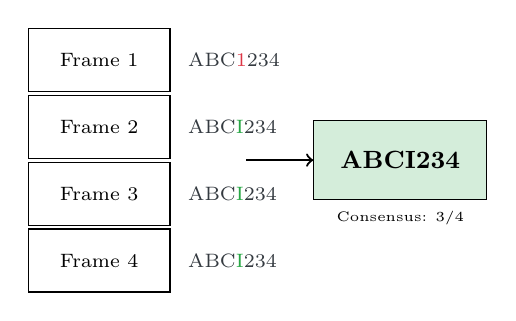
\begin{tikzpicture}[scale=0.85]
    % Frame boxes
    \node[draw, minimum width=1.8cm, minimum height=0.8cm, font=\scriptsize] (f1) at (0,4) {Frame 1};
    \node[right=0.1cm of f1, font=\scriptsize, color=darkgray] {ABC\textcolor{criticalred}{1}234};

    \node[draw, minimum width=1.8cm, minimum height=0.8cm, font=\scriptsize] (f2) at (0,3) {Frame 2};
    \node[right=0.1cm of f2, font=\scriptsize, color=darkgray] {ABC\textcolor{safegreen}{I}234};

    \node[draw, minimum width=1.8cm, minimum height=0.8cm, font=\scriptsize] (f3) at (0,2) {Frame 3};
    \node[right=0.1cm of f3, font=\scriptsize, color=darkgray] {ABC\textcolor{safegreen}{I}234};

    \node[draw, minimum width=1.8cm, minimum height=0.8cm, font=\scriptsize] (f4) at (0,1) {Frame 4};
    \node[right=0.1cm of f4, font=\scriptsize, color=darkgray] {ABC\textcolor{safegreen}{I}234};

    % Arrow
    \draw[->, thick] (2.2,2.5) -- (3.2,2.5);

    % Result
    \node[draw, fill=safegreen!20, minimum width=2.2cm, minimum height=1cm, font=\small\bfseries] at (4.5,2.5) {ABCI234};
    \node[below=0.1cm, font=\tiny] at (4.5,2) {Consensus: 3/4};
\end{tikzpicture}

\vspace{0.5cm}
\begin{center}
\begin{tabular}{lcc}
\toprule
\textbf{Method} & \textbf{Accuracy} \\
\midrule
Single-frame & 71.3\% \\
Multi-frame (ours) & \highlight{89.7\%} \\
\bottomrule
\end{tabular}
\end{center}
\end{column}
\end{columns}
\end{frame}

% ============================================================================
% RESULTS
% ============================================================================
\begin{frame}{Results: System Performance}
\begin{columns}[T]
\begin{column}{0.5\textwidth}
\textbf{Detection \& Tracking}
\begin{itemize}
    \item YOLOv10: \highlight{94.2\%} mAP@0.5
    \item ByteTrack: \highlight{<5\%} ID switches
    \item Passenger filtering: \highlight{99\%} reduction in false positives
\end{itemize}

\vspace{0.4cm}
\textbf{Collision Prediction}
\begin{center}
\begin{tabular}{lccc}
\toprule
& \textbf{P} & \textbf{R} & \textbf{F1} \\
\midrule
Critical & 0.87 & 0.92 & 0.89 \\
Warning & 0.79 & 0.85 & 0.82 \\
\bottomrule
\end{tabular}
\end{center}
\end{column}
\begin{column}{0.5\textwidth}
\textbf{Latency (RTX 3080)}
\begin{center}
\begin{tikzpicture}
\begin{axis}[
    xbar,
    width=6cm,
    height=5cm,
    bar width=10pt,
    xlabel={Latency (ms)},
    symbolic y coords={LPR, Ground Plane, Risk, Tracking, Detection},
    ytick=data,
    y tick label style={font=\scriptsize},
    xmin=0,
    xmax=550,
    nodes near coords,
    nodes near coords style={font=\tiny},
]
\addplot[fill=accentblue!70] coordinates {
    (75, Detection)
    (25, Tracking)
    (8, Risk)
    (40, Ground Plane)
    (400, LPR)
};
\end{axis}
\end{tikzpicture}
\end{center}

\vspace{0.2cm}
\centering
\highlight{10+ FPS} real-time throughput
\end{column}
\end{columns}
\end{frame}

% ============================================================================
% EARLY WARNING
% ============================================================================
\begin{frame}{Results: Early Warning Capability}
\begin{center}
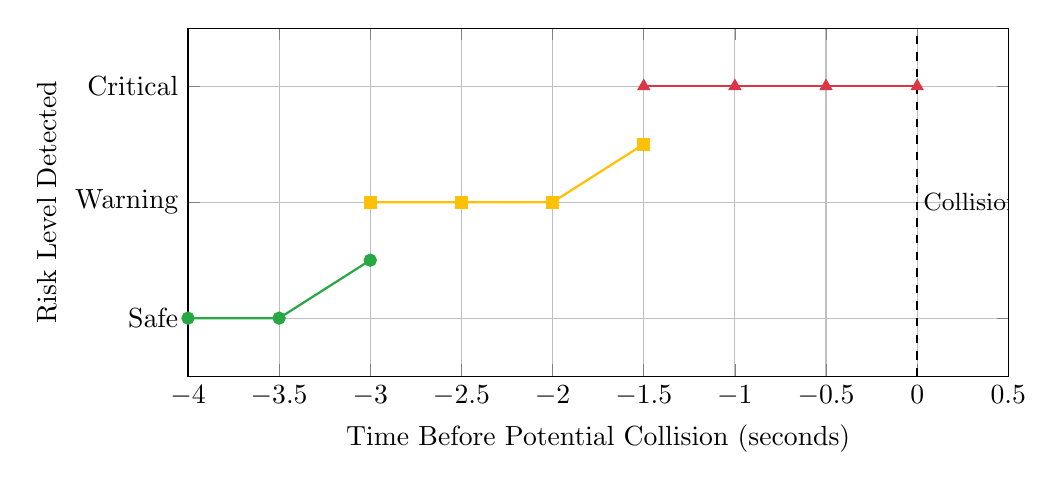
\begin{tikzpicture}
\begin{axis}[
    width=12cm,
    height=6cm,
    xlabel={Time Before Potential Collision (seconds)},
    ylabel={Risk Level Detected},
    ytick={1,2,3},
    yticklabels={Safe, Warning, Critical},
    xmin=-4,
    xmax=0.5,
    ymin=0.5,
    ymax=3.5,
    grid=major,
    legend pos=north west,
]
% Risk level over time
\addplot[thick, color=safegreen, mark=*] coordinates {
    (-4, 1)
    (-3.5, 1)
    (-3, 1.5)
};
\addplot[thick, color=warningorange, mark=square*] coordinates {
    (-3, 2)
    (-2.5, 2)
    (-2, 2)
    (-1.5, 2.5)
};
\addplot[thick, color=criticalred, mark=triangle*] coordinates {
    (-1.5, 3)
    (-1, 3)
    (-0.5, 3)
    (0, 3)
};
% Collision point
\draw[dashed, thick] (axis cs:0,0.5) -- (axis cs:0,3.5);
\node[font=\small] at (axis cs:0.3,2) {Collision};
\end{axis}
\end{tikzpicture}
\end{center}

\begin{center}
\Large
\safe{3.0s} Warning alert \quad$\rightarrow$\quad \critical{1.5s} Critical alert
\end{center}
\end{frame}

% ============================================================================
% DEMO VIDEO
% ============================================================================
\begin{frame}{System in Action}
\begin{center}
\begin{tikzpicture}
    % Video frame placeholder
    \draw[thick, fill=lightgray] (0,0) rectangle (10,5.6);
    \node[font=\Large] at (5,2.8) {\faPlayCircle\quad Live Demo};

    % Annotations
    \node[draw, fill=safegreen!30, rounded corners, font=\scriptsize] at (2,4.5) {Pedestrian: ID 5};
    \node[draw, fill=criticalred!30, rounded corners, font=\scriptsize] at (8,4.5) {Vehicle: ID 12};

    % Risk indicator
    \node[draw, fill=warningorange, rounded corners, font=\small\bfseries, text=white] at (5,0.7) {WARNING: TTC 2.3s};
\end{tikzpicture}
\end{center}

\textbf{Key Visualizations:}
\begin{itemize}
    \item Bounding boxes with track IDs
    \item Real-time risk tier overlays
    \item Trajectory predictions
    \item License plate readouts
\end{itemize}
\end{frame}

% ============================================================================
% ARCHITECTURE BENEFITS
% ============================================================================
\begin{frame}{Architecture Benefits}
\begin{columns}[T]
\begin{column}{0.5\textwidth}
\textbf{Modularity}
\begin{itemize}
    \item Each component independently testable
    \item Easy to upgrade individual modules
    \item Clean interfaces between stages
\end{itemize}

\vspace{0.4cm}
\textbf{Flexibility}
\begin{itemize}
    \item Fixed and PTZ camera support
    \item YAML-based configuration
    \item Multiple deployment modes
\end{itemize}
\end{column}
\begin{column}{0.5\textwidth}
\textbf{Robustness}
\begin{itemize}
    \item Multi-method fallbacks
    \item Graceful degradation
    \item Temporal smoothing
\end{itemize}

\vspace{0.4cm}
\textbf{Extensibility}
\begin{itemize}
    \item Plugin architecture for new detectors
    \item VLM escalation hooks
    \item Depth estimation integration
\end{itemize}
\end{column}
\end{columns}

\vspace{0.5cm}
\begin{center}
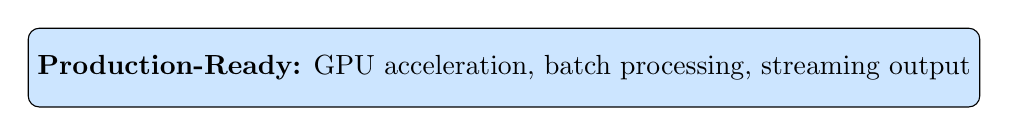
\begin{tikzpicture}
    \node[draw, rounded corners, fill=accentblue!20, minimum width=10cm, minimum height=1cm] {
        \textbf{Production-Ready:} GPU acceleration, batch processing, streaming output
    };
\end{tikzpicture}
\end{center}
\end{frame}

% ============================================================================
% FUTURE WORK
% ============================================================================
\begin{frame}{Future Work}
\begin{columns}[T]
\begin{column}{0.5\textwidth}
\textbf{Phase 2: Impact Detection}
\begin{itemize}
    \item Velocity discontinuity analysis
    \item Fall-like motion detection
    \item Track disappearance signals
\end{itemize}

\vspace{0.4cm}
\textbf{Phase 3: VLM Escalation}
\begin{itemize}
    \item Vision-Language Model verification
    \item Reduced false positives
    \item Semantic scene understanding
\end{itemize}
\end{column}
\begin{column}{0.5\textwidth}
\textbf{Phase 4: Advanced Prediction}
\begin{itemize}
    \item Learning-based trajectory forecasting
    \item Social force models
    \item Intent prediction
\end{itemize}

\vspace{0.4cm}
\textbf{Research Directions}
\begin{itemize}
    \item Monocular depth integration
    \item Cross-camera tracking
    \item Real-time deployment at scale
\end{itemize}
\end{column}
\end{columns}
\end{frame}

% ============================================================================
% CONCLUSION
% ============================================================================
\begin{frame}{Conclusion}
\begin{columns}[T]
\begin{column}{0.6\textwidth}
\textbf{We presented \textsc{NearMiss}:}
\begin{enumerate}
    \item Real-time collision risk assessment system
    \item Novel calibration-free ground plane estimation
    \item Physics-based prediction with CPA
    \item Multi-frame OCR aggregation for reliable LPR
\end{enumerate}

\vspace{0.4cm}
\textbf{Key Results:}
\begin{itemize}
    \item \highlight{1.5--3 seconds} advance warning
    \item \highlight{89\%} F1 on critical risk detection
    \item \highlight{10+ FPS} real-time performance
    \item \highlight{90\%} license plate accuracy
\end{itemize}
\end{column}
\begin{column}{0.4\textwidth}
\begin{center}
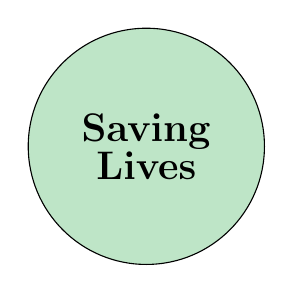
\begin{tikzpicture}
    \node[draw, circle, fill=safegreen!30, minimum size=3cm, align=center] {
        \Large\textbf{Saving}\\
        \Large\textbf{Lives}
    };
\end{tikzpicture}

\vspace{0.5cm}
\textit{``Technology should serve humanity.''}
\end{center}
\end{column}
\end{columns}
\end{frame}

% ============================================================================
% QUESTIONS
% ============================================================================
\begin{frame}[standout]
Questions?

\vspace{1cm}
\normalsize
\faEnvelope\quad veer19297@gmail.com

\faGithub\quad github.com/InspiritAI/Near-Miss-Detection
\end{frame}

% ============================================================================
% BACKUP SLIDES
% ============================================================================
\appendix

\begin{frame}{Backup: ByteTrack Algorithm Details}
\textbf{Two-Stage Association:}
\begin{enumerate}
    \item Match high-confidence detections ($>0.5$) with tracks using IoU
    \item Match remaining tracks with low-confidence detections ($0.1$--$0.5$)
\end{enumerate}

\vspace{0.5cm}
\textbf{Track Lifecycle:}
\begin{itemize}
    \item \textbf{Tentative}: New detection, needs confirmation
    \item \textbf{Confirmed}: Matched for $\geq3$ consecutive frames
    \item \textbf{Lost}: No match for $N$ frames, kept in buffer
    \item \textbf{Deleted}: Lost for $>30$ frames
\end{itemize}

\vspace{0.3cm}
\textbf{Why ByteTrack?}
\begin{itemize}
    \item Recovers occluded objects via low-confidence detections
    \item No appearance features needed (fast)
    \item State-of-the-art on MOT benchmarks
\end{itemize}
\end{frame}

\begin{frame}{Backup: CPA Mathematical Derivation}
\textbf{Setup:}
\begin{itemize}
    \item Pedestrian: position $\mathbf{p}_p$, velocity $\mathbf{v}_p$
    \item Vehicle: position $\mathbf{p}_v$, velocity $\mathbf{v}_v$
    \item Relative position: $\mathbf{r} = \mathbf{p}_p - \mathbf{p}_v$
    \item Relative velocity: $\mathbf{w} = \mathbf{v}_p - \mathbf{v}_v$
\end{itemize}

\vspace{0.3cm}
\textbf{Derivation:}
\begin{align*}
\text{Distance at time } t: \quad d(t) &= |\mathbf{r} + t\mathbf{w}| \\
\text{Minimize } d^2(t): \quad \frac{d}{dt}|\mathbf{r} + t\mathbf{w}|^2 &= 0 \\
2(\mathbf{r} + t\mathbf{w}) \cdot \mathbf{w} &= 0 \\
t_{CPA} &= -\frac{\mathbf{r} \cdot \mathbf{w}}{|\mathbf{w}|^2}
\end{align*}

\vspace{0.3cm}
\textbf{Edge Cases:}
\begin{itemize}
    \item $|\mathbf{w}| \approx 0$: Objects moving in parallel, use current distance
    \item $t_{CPA} < 0$: Objects diverging, closest approach was in the past
\end{itemize}
\end{frame}

\begin{frame}{Backup: Homography-Based Ground Plane}
\begin{columns}[T]
\begin{column}{0.5\textwidth}
\textbf{From Vanishing Point to Homography:}
\begin{enumerate}
    \item Detect lane markings (Canny + Hough)
    \item Find vanishing point (line intersection)
    \item Define 4-point correspondence:
    \begin{itemize}
        \item Image corners
        \item Ground plane corners (10m $\times$ 20m)
    \end{itemize}
    \item Compute homography matrix $H$
\end{enumerate}

\vspace{0.3cm}
\textbf{Coordinate Transform:}
\begin{equation*}
\begin{pmatrix} x' \\ y' \\ 1 \end{pmatrix} = H \begin{pmatrix} u \\ v \\ 1 \end{pmatrix}
\end{equation*}
\end{column}
\begin{column}{0.5\textwidth}
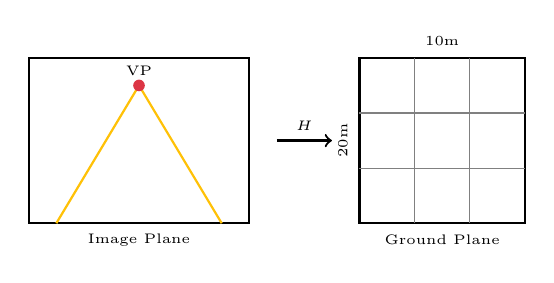
\begin{tikzpicture}[scale=0.7]
    % Image plane
    \draw[thick] (0,0) -- (4,0) -- (4,3) -- (0,3) -- cycle;
    \node[font=\tiny] at (2,-0.3) {Image Plane};

    % Lane lines
    \draw[thick, color=warningorange] (0.5,0) -- (2,2.5);
    \draw[thick, color=warningorange] (3.5,0) -- (2,2.5);

    % Vanishing point
    \fill[color=criticalred] (2,2.5) circle (3pt);
    \node[font=\tiny, above] at (2,2.5) {VP};

    % Arrow
    \draw[->, thick] (4.5,1.5) -- (5.5,1.5);
    \node[font=\tiny, above] at (5,1.5) {$H$};

    % Ground plane (bird's eye)
    \begin{scope}[shift={(6,0)}]
        \draw[thick] (0,0) -- (3,0) -- (3,3) -- (0,3) -- cycle;
        \node[font=\tiny] at (1.5,-0.3) {Ground Plane};

        % Grid
        \draw[thin, color=gray] (1,0) -- (1,3);
        \draw[thin, color=gray] (2,0) -- (2,3);
        \draw[thin, color=gray] (0,1) -- (3,1);
        \draw[thin, color=gray] (0,2) -- (3,2);

        % Scale
        \node[font=\tiny] at (1.5,3.3) {10m};
        \node[font=\tiny, rotate=90] at (-0.3,1.5) {20m};
    \end{scope}
\end{tikzpicture}
\end{column}
\end{columns}
\end{frame}

\end{document}
